\subsubsection{Third article}

The purpose of the article "Fixbi: Bridging domain spaces for unsupervised domain adaptation" written by Jaemin Na, Heechul Jung et al. \cite{na2021fixbi} is to propose a  fixed ratio-based mixup method to address the problem of large domain discrepancies. The authors mix up images and then fed them into neural networks to achieve greater reliability in learning from corrupted labels. It is proposed to use two predetermined mixup ratios $\lambda_sd$ and $\lambda_td$ for the source and target domain respectively. 
Denote input samples and their labels for source and target domain as $(x_i^s, y_i^s)$ and $(x_i^t, \hat{y}_i^t)$, the authors define mixup configurations in the following way:

\begin{equation*}
\begin{split}
 \tilde{x}^{st}_i &= \lambda x_i^s + (1 - \lambda)x_i^t\\
 \tilde{y}^{st}_i &= \lambda y_i^s + (1 - \lambda)\hat{y}_i^t,
\end{split}
\end{equation*} 

where $\lambda \in \{\lambda_{sd}, \lambda_{td} \}$ and $\lambda_{sd} + \lambda_{td} = 1$, $\hat{y}_i^t$ is the pseudo-labels for the target samples. By leveraging the fixed ratio-based mixup, it is constructed two neural networks with different perspectives: the "source-dominant model" (SDM) and the "target-dominant model" (TDM) (see Figure \ref{fig: fixbi}).

\begin{figure}[H]
    \centering
    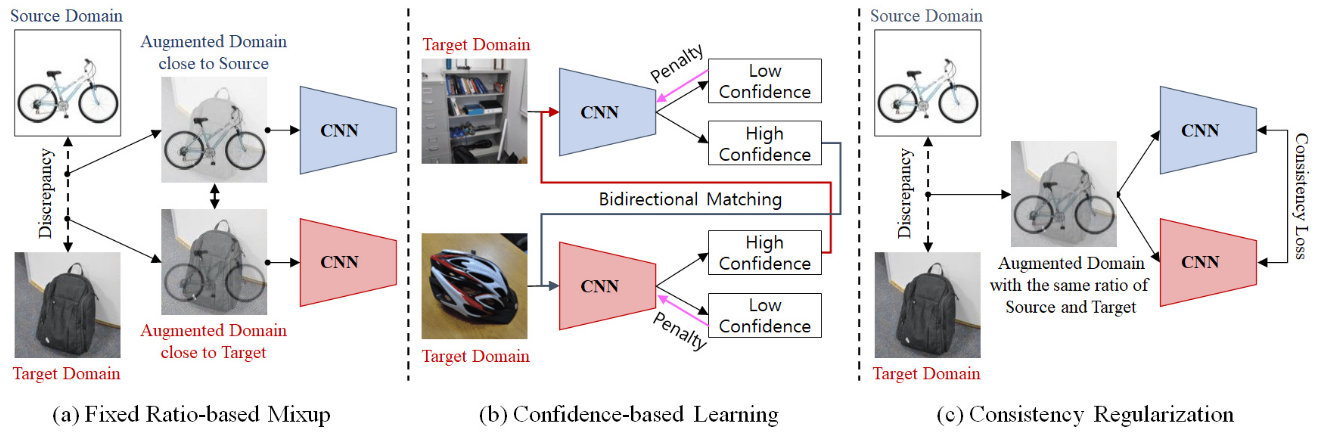
\includegraphics[width=\textwidth]{Figures/From articles/fixbi.png}
    \caption{All parts of FixBi training model: (a) fixed ratio-based mixup, (b)
confidence-based learning and (c) consistency regularization.}
    \label{fig: fixbi}
\end{figure}

The SDM provides robust supervision for the source domain but relatively weak supervision for the target domain, while the TDM has strong supervision for the target domain but weaker supervision for the source domain. Thus, denoting $p(y| \tilde{x}^{st}_i)$ as a predicted class distribution, it is defined fixed ratio-based mixup function 

$$
L_{fm} = \dfrac{1}{B} \sum_{i = 1}^B \hat{y}^{st}_i \log (p(y|\tilde{x}^{st}_i)),
$$

where $\hat{y}^{st}_i = \arg \max p(y|\tilde{x}^{st}_i)$ and $B$ is the size of a mini-batch. In order to have connections between source and target domains, it is suggested to use a confidence-based learning approach whereby one model educates the other using positive pseudo-labels, or penalties itself using negative pseudo-labels. Positive pseudo-labels means labels which predictions are above a specific threshold, then the authors use them in training the second model by utilizing a conventional cross-entropy loss. Thus, denote p and q as distributions of two models, the authors get the following loss function

$$
L_{bim} = \dfrac{1}{B}\sum_{i=1}^B \mathds{1}(\max (p(y|x_i^t) > \tau)\hat{y}_i^t \log (q(y|x_i^t)),
$$
where $\hat{y}_i^t = \arg \max p(y|x_i^t)$. In contrast, a negative pseudo-label refers to the top-1 label predicted by the network with a confidence below the threshold $\tau$. The function of self-penalization is defined as follows:

$$
L_{sp} = \dfrac{1}{B}\sum_{i=1}^B \mathds{1}(\max (p(y|x_i^t) < \tau)\hat{y}_i^t \log (1 - p(y|x_i^t))
$$
Furthermore, the threshold is changed adaptively during training. In addition, it is introduced the following expression: 

$$
L_{cr} = \dfrac{1}{B} \sum_{i=1}^B \| p(y|\tilde{x}^{st}_i) - q(y|\tilde{x}^{st}_i)\|^2_2
$$
that represents consistency regularization to guarantee a stable convergence during the training of both models.